\documentclass[a4paper,14pt]{extreport}
\usepackage[utf8]{inputenc} % Set Encoding
\usepackage[T1,T2A]{fontenc}
\usepackage{fontspec} % Using custom fonts (requires -xelatex flag)
\usepackage[russian,english,ukrainian]{babel} % Using languages
\usepackage[left=3cm, right=2cm, top=2cm, bottom=2cm]{geometry}
\usepackage[raggedright]{titlesec} % For section modification
\usepackage{indentfirst} % Inserts indents in paragraphs
\usepackage{minted} % For code listing
\usepackage{graphicx} % For image insertions
\usepackage{float} % For positioning
\usepackage[section]{placeins}
\usepackage{fancyhdr}
\usepackage[tableposition=bottom,singlelinecheck=false]{caption} % captions in figures and tables
\usepackage{enumitem} % List indents
\usepackage{chngcntr}
\usepackage[english,russian,ukrainian]{babel}
% \usepackage[nottoc]{tocbibind}
\usepackage{color}
\usepackage{xpatch}
\definecolor{spot}{rgb}{0,0,0}
\usepackage[colorlinks,allcolors=spot,bookmarksopen=true,pdfstartview=FitH]{hyperref}
\usepackage{amsmath}
\usepackage{etoolbox}% vspace before and after figure
\usepackage[normalem]{ulem} %for uline
\usepackage{subcaption} % for multiple dependent pics
\usepackage{titletoc}
\usepackage{multirow} % advanced table formatting
\usepackage[title,titletoc]{appendix} % appendings
\usepackage{array}
\usepackage{amsfonts}
\usepackage{mfirstuc}

\AtBeginEnvironment{figure}{\vspace{0.5em}}
\AtEndEnvironment{figure}{\vspace{\baselineskip}}

\AtBeginEnvironment{equation}{\vspace{0.5em}}
\AtEndEnvironment{equation}{\vspace{\baselineskip}}

% \AtBeginEnvironment{aligned}{\vspace{\baselineskip}}
% \AtEndEnvironment{aligned}{\vspace{\baselineskip}}

% \AtBeginEnvironment{gather}{\vspace{\baselineskip}}
% \AtEndEnvironment{gather}{\vspace{\baselineskip}}

\AtBeginEnvironment{table}{\vspace{0.5em}}
\AtEndEnvironment{table}{\vspace{\baselineskip}}

\newcommand\tline[2]{$\underset{\text{#1}}{\text{\underline{\hspace{#2}}}}$}% line with underset

% PAGE NUMBERING
\pagestyle{fancy}
\fancyhf{}
\rhead{\thepage}
\renewcommand{\headrulewidth}{0pt}

\pagenumbering{gobble}

\linespread{1.3} % 1.5 spacing between lines

\setlength\parindent{5ex} % paragraph indents

\fancypagestyle{plain}{ 
  \fancyhf{}
  \rhead{\thepage}}

% CHAPTER FORMATTING
\titleformat{\chapter}[block] % chapter style
  {\filcenter}
  {\thechapter}
  {1em}
  {\MakeUppercase}{}
\titlespacing*{\chapter}{0pt}{-30pt}{*4} 

% SECTION FORMATTING
\titleformat{\section}
  {}
  {\thesection}
  {1ex}{}
\titlespacing*{\section}{\parindent}{*4}{*4}
\titleformat{\subsection}
  {}
  {\thesubsection}
  {1ex}{}
\titlespacing*{\subsection}{\parindent}{*4}{*4}
\titleformat{\subsubsection}
  {}
  {\thesubsubsection}
  {1ex}{}
\titlespacing*{\subsubsection}{\parindent}{*4}{*4}
% CREATE COMMAND ALLOWS UNNUMBERED CHAPTER APPEAR IN TABLE OF CONTENTS
\newcommand\uchapter[1]{%
  \chapter*{#1}%
  \addcontentsline{toc}{chapter}{\xmakefirstuc{\lowercase{#1}}}}

% MAKE IT UKRAINIAN
% \addto{\captionsrussian}{\renewcommand*{\contentsname}{Содержание}}

% NO SPACING BEFORE TOC HEADING
\dottedcontents{chapter}[1.6em]{}{1.6em}{1pc}

% NORMAL CAPTIONS
\DeclareCaptionLabelFormat{gostfigure}{Рисунок #2}
\DeclareCaptionLabelFormat{gosttable}{Таблиця #2}
\DeclareCaptionLabelSeparator{gost}{~---~}
\captionsetup{labelsep=gost}
\captionsetup*[figure]{labelformat=gostfigure}
\captionsetup*[table]{labelformat=gosttable}
\renewcommand{\thesubfigure}{\asbuk{subfigure}}

% PADDINGS IN TABLES
\renewcommand{\arraystretch}{1.3}

% CENTERED IMAGE CAPTIONS
\captionsetup*[figure]{labelformat=gostfigure, justification=centering}

\setcounter{secnumdepth}{4}

% % PROPER LISTS SETUP
\makeatletter
    \AddEnumerateCounter{\asbuk}{\@asbuk}{ю)}
\makeatother
\setlist{nolistsep}
\renewcommand{\labelitemi}{-}
\renewcommand{\labelenumi}{\alph{enumi})}
\renewcommand{\labelenumii}{\alpha{enumii})}
\setenumerate{leftmargin=\parindent}

% EXPLANATIONS IN FOOTER
\renewcommand*{\thefootnote}{\arabic{footnote})}
\renewcommand{\footnoterule}{%
  \kern -3pt
  \hrule width 40mm height .4pt
  \kern 2.6pt
}

% DISABLE WORD SPLITTING IN HEADINGS
\titleformat*{\section}{\sloppy\righthyphenmin62}

% ONE SPACE AFTER DOT
\frenchspacing

% FONTS
\setmainfont{Liberation Serif} % Set default font on Linux

% WIDELINE
\newcommand{\wideunderline}[2][2em]{%
  \underline{\makebox[\ifdim\width>#1\width\else#1\fi]{#2}}%
}

\setlength{\headheight}{17.0pt}

\graphicspath{{./pics}}

\newcommand{\StundentNameRod}{Соколенка Д. О.}
\newcommand{\StundentName}{Соколенко Д. О.}
\newcommand{\University}{Харківський національний університет радіоелектроніки}
\newcommand{\StundentFullName}{Соколенко Дмитро Олександрович}
\newcommand{\Department}{штучного інтелекту}
\newcommand{\Topic}{Transformers for Image Recognition at Scale}
\newcommand{\Grade}{3}
\newcommand{\Group}{ІТШІ-18-1}
\newcommand{\Faculty}{КН}
\newcommand{\Speciality}{Комп'ютерні науки}
\newcommand{\SpecialityCode}{122}
\newcommand{\Graduate}{бакалавр}
\newcommand{\ScientificDirectorName}{Вітько О. В.}
\newcommand{\ScientificDirectorNameFull}{Вітько Вітько Олександра Валеріївна}
\newcommand{\ScientificDirectorPosition}{доцент каф. ШІ, доц., к.т.н.}
\newcommand{\ScientificDirectorPositionSmall}{к.т.н, доц.}
\newcommand{\MemberCommisionF}{Вітько О. В.}
\newcommand{\MemberCommisionS}{Кулішова Н. Є.}
\newcommand{\MemberCommisionT}{Бібічков І. Є.}


\begin{document}
\begin{titlepage}
    \setlength\parindent{0pt}
    \centering

    \University

    \vspace{1.5ex}

    Кафедра \Department
    
    \vspace{10ex}

    \uppercase{\textbf{міждисциплінарний \\ курсовий проект}}

    \vspace{4ex}

    на тему: <<\Topic>>

    \vspace{4cm}
    \hfill
    \begin{minipage}{9cm}
        \begin{flushleft}
            
            Студента \uline{\hfill\Grade\hfill}
            курсу групи \uline{\hfill\Group\hfill} \\
            спеціальності \uline{\hfill\Speciality\hfill} \\
            \uline{\hfill\StundentName\hfill} \\
            \vspace{1ex}
            Керівник \uline{\hfill\ScientificDirectorPosition\hfill} \\
            \uline{\hfill\ScientificDirectorName\hfill} \\
            \vspace{3ex}
            Національна шкала: \uline{\hfill} \\ 
            \vspace{1ex}
            Кількість балів: \uline{\hfill} Оцінка ECTS \uline{\hfill}
        \end{flushleft}
    \end{minipage}

    \vspace{9ex}
    \hfill
    \begin{minipage}{13cm}
        \begin{flushright}
            Члени коміссії \hspace{.7cm}
            $\underset{\text{(підпис)}}{\underline{\hspace{3cm}}}$ \hspace{.5em}
            \wideunderline[10em]{\MemberCommisionF} \\
            $\underset{\text{(підпис)}}{\underline{\hspace{3cm}}}$ \hspace{.5em}
            \wideunderline[10em]{\MemberCommisionS} \\
            $\underset{\text{(підпис)}}{\underline{\hspace{3cm}}}$ \hspace{.5em}
            \wideunderline[10em]{\MemberCommisionT} \\
        \end{flushright}
    \end{minipage}
    
    \vfill
	{Харків \the\year{}}
\end{titlepage}

\thispagestyle{empty}
{
    \setlength\parindent{0pt}
    \linespread{2}

    \uline{\hfill\University\hfill}
    \vspace{1ex}

    Інститут, \uline{факультет}, відділення \hspace{1em} \uline{\hfill\Speciality\hfill} 
    \vspace{.5ex}

    \uline{Кафедра}, циклова комісія \hspace{1em} \uline{\hfill\Department\hfill}
    \vspace{.5ex}
    
    Освітньо кваліфікаційний рівень \hspace{1em} \uline{\hfill\Graduate\hfill}
    \vspace{.5ex}

    Спеціальність \hspace{1em} \uline{\hfill\SpecialityCode <<\Speciality>>\hfill}
    
    \vspace{5ex}
    \hfill
    \begin{minipage}{11cm}
        \begin{flushright}
            \uppercase{\textbf{Затверджую}} \\
            \textbf{Завідувач кафедри} \uline{\hfill} \\
            \hspace{2cm}\uline{\hfill} \\
            \hspace{2cm}``\underline{\hspace{1cm}''}\uline{\hfill} \hspace{.5cm} {\the\year{}}

        \end{flushright}
    \end{minipage}
    
    \vfill
    {
        \centering
        \uppercase{\textbf{\large{завдання}}}
        
        \uppercase{\textbf{на міждисциплінарний курсовий проект}}

        \uline{\hfill$\underset{\text{(прізвище, ім'я, по батькові)}}{\text{\StundentFullName}}$\hfill}}
        \vspace{0.5em}
        % $\underset{\text{(прізвище, ім'я, по батькові)}}{\uline{\hfill\text{\StundentFullName}}}$

        1. Тема проекту \uline{\hfill\Topic\hfill}

        Керівник проекту \uline{\hfill\ScientificDirectorNameFull, \ScientificDirectorPositionSmall\hfill}

        2. Строк подання студентом проекту \uline{\hfill10.06.2021\hfill}
        
        3. Вихідні дані до проекту \uline{An Image is Worth 16x16 Words: Transformers\hfill}

        \uline{for Image Recognition at Scale, A. Dosovitskiy, L. Beyer, A. Kolesnikov та ін.; Python; Transformers; Image recognition\hfill}

        \uline{\hfill}

        \uline{\hfill}

        4. Зміст розрахунково-пояснювальної записки (перелік питань, які підлягають розробці)
        \uline{Аналіз предметної області, Теоретичні дослідження,\hfill}

        \uline{Експериментальні дослідження\hfill}

        \uline{\hfill}
        
        \uline{\hfill}

        5. Дата видачі завдання \uline{\hfill 22.04.2021 \hfill}
}

\newpage
\thispagestyle{empty}
{
    \setlength\parindent{0pt}

    \begin{center}
        \uppercase{Клендарний план}
    \end{center}

    \begin{tabular}{ | m{0.8cm} | m{9.5cm}| m{3cm} | m{2.5cm} | } 
        \hline
        № & Назва етапів проектів & Термін виконання етапів проекту & Примітка \\
        \hline
        1 & Аналіз літератури та інтернет-джерел & 01.06-05.06 & Виконано\\
        \hline
        2 & Постановка задачі, узгодженя з керівником & 05.06-08.06 & Виконано\\
        \hline
        3 & Проведення теоретичних досліджень & 08.06-10.06 & Виконано\\
        \hline
        4 & Проведення експериментальних досліджень & 10.06-15.06 & Виконано\\
        \hline
        5 & Аналіз результатів, що отримані під час виконання роботи & 15.06-16.06 & Виконано\\
        \hline
        6 & Оформлення презентації курсового проєкту & 16.06-17.06 & Виконано\\
        \hline
        7 & Подання пояснювальної записки на перевірку & За 1 день до захисту & Виконано\\
        \hline
        8 & Захист МКП & 18.06 & Виконано\\
        \hline
    \end{tabular}

    \vspace{8ex}

    \hfill
    \begin{minipage}{12cm}
        \begin{flushright}
            \textbf{Студент}
            \tline{Підпис}{1.5cm} \hspace{.5em}
            \wideunderline[10em]{\StundentName} \\
            \textbf{Керівник проекту}
            \tline{Підпис}{1.5cm} \hspace{.5em}
            \wideunderline[10em]{\ScientificDirectorName} \\
        \end{flushright}
    \end{minipage}
}

\newpage
\chapter*{Реферат}
Пояснювальна записка: 38с., 10 рис., 3 табл., 25 джерел, 1 додаток.

\vspace{\baselineskip}

ШТУЧНА НЕЙРОННА МЕРЕЖА, ТРАНСФОРМЕР,
УВАГА, БАГАТОГОЛОВКОВА УВАХА, МАШИННЕ НАВЧАННЯ,
МАШТАБУВАННЯ, КЛАСИФІКАЦІЯ ЗОБРАЖЕНЬ,
ПОПЕРЕДНЄ ТРЕНУВАННЯ.

\vspace{\baselineskip}

Об’єкт дослідження -- застосування архітектури
трансформера до задачі класифікації зображень.

Мета роботи -- набути навичок читання зарубіжної наукової літератури та аналізу наукових статей. Навчитися робити висновки з нової інформації.

Метод дослідження: проведення теоретичних та експериментальних досліджень.

Одержані висновки та їх новизна: трансформер є достатньо загальною
архітектурою, яка може успішно використовуватися для вирішення задач
класифікації зображень, якщо є достатньо даних та обчислювальних ресурсів.
Трансформер показує себе краще найкращіх сучасних методів, заснованих на
згорткових мережах, якщо його натренувати на достатньо великому датасеті,
а потім точно налаштувати під конкретну задачу.

\newpage
\tableofcontents

\newpage
\chapter*{Перелік умовних позначень, символів, одиниць, скорочень та термінів}
ГНМ -- Глибокі нейронні мережі

РНМ -- Рекурентні нейронні мережі

ЗНМ -- Згорткові нейронні мережі



\newpage
\pagenumbering{arabic}
\setcounter{page}{7}
\uchapter{ВСТУП}
З ростом обчислювальних можливостей, об'ємів пам'яті у комп'ютерах
з'явився потенціал в моделях машинного навчання, які мають
великі простіри гіпотез, та мільйони параметрів для навчання.
Такі моделі завдяки своїй складності можуть наближено представляти
довільні функції, такі як переклад з однієї мови на іншу,
розпізнавання об'єктів на зображенні, опис зображень,
генерація нових зображень, розміння мови, та інші.

Нейронні мережі успішно застосовуються в багатьох галузях
завдяки своїм репрезентативним можливостям. Для кожної задачі
існує архітектура мережі, яка найбільш гарно вірішує поставлену
проблему, але для інших не пов'язаних між собою задач вона
показує себе гірше, ніж спеціальні архітектури, розроблені
для тих чи інших проблем. Проте загальні архітектури,
які можуть вирішувати декілька поставлених задач, мають
перевагу над спеціалізованими архітектурами, так як їх
можна використовувати для навчання з переходом на інший домен,
тим самим дозволяючи навчити модель на загальному датасеті,
який містить багато даних,
та потім налаштувати модель для виконання задачі, яка не має такої
кількості даних. Це дозволяє вирішувати складні задачі, де
нові дані складно або довго отримати.

Зокрема, архітектура трансформера є більш загальною моделлю,
ніж рекурентні мережі, та згорткові мережі. Вона не містить
у собі тих припущень,
що корисні для вирішення задач обробки природної мови, або
роботи з зображеннями. Трансформери початково були створені
для вирішення задачі машинного перекладу без використання
рекурентності, та в цій роботі ми демонструємо, що
трансформери також можуть вирішувати задачу класифікації зображень
з мінімальними модифікаціями, не використовуючи згорткові шари.

\newpage
\chapter{Аналіз предметної галузі}
% https://papers.nips.cc/paper/2014/file/a14ac55a4f27472c5d894ec1c3c743d2-Paper.pdf
Глибокі нейронні мережі (ГНМ) -- надзвичайно потужні моделі машинного навчання,
які досягають чудової точності у таких складних задачах, як
розпізнавання мови та візуальне розпізнавання об’єктів.
ГНМ є потужними, оскільки вони можуть виконувати
довільні паралельні обчислення за невелику кількість кроків.
Отже, хоча нейронні мережі пов’язані
зі звичайними статистичними моделями, вони вивчають складні
обчислення. Більше того, великі ГНМ можна навчати зі
зворотним розповсюдженням, коли мічений навчальний набір має
достатньо інформації для визначення параметрів мережі. Таким
чином, якщо існує параметр великого ГНМ, який досягає хороших
результатів (наприклад, оскільки люди можуть вирішити завдання
дуже швидко), зворотне розповсюдження знайде ці
параметри і вирішить проблему.

\section{Штучні нейронні мережі}
Штучна нейронна мережа побудована навколо біологічної метафори.
Будова первинної зорової кори відносно добре відома,
і вчені виграли Нобелівську премію з фізіології за відкриття в
1962 р. організації нейронів у перших кортикальних
шарах \cite{cortex-stuff}. Таким чином, в надзвичайно
спрощеному вигляді
мозку нейрони організовані шарами, кожен нейрон отримує
інформацію з попереднього шару, виконує дуже просте
обчислення і передає свій результат нейронам наступного
шару. Однак слід пам’ятати, що це лише метафора та джерело
натхнення: біологічні мережі мають набагато складніші
зв’язки, а математичні рівняння, що керують ними, також
є більш складними \cite{cortex-equations}.

\subsection{Перцептрон}
Перцептрони -- винайдені Френком Розенблаттом у 1957 році
\cite{rozenblatt}, є найпростішою
нейронною мережею, яка складається з $n$ кількості входів, лише одного
нейрона та одного виходу, де $n$ - кількість рис нашого набору
даних. Процес вираховухання результату класифікації починається
з обчислення зваженої суми
по формулі \ref{eq:perceptron1}.

\begin{equation}
    z = \sum^n_{i=1} x_i w_i + b
    \label{eq:perceptron1}
\end{equation}

де $w$ -- вектор дійсних ваг, $b$ -- зміщення.
Коефіцієнт зміщення зміщує межу прийняття рішення
від початку координат і не залежить від будь-якого
вхідного значення.

Потім на зваженій сумі використовується функція активації.

\begin{equation}
    \phi(z) = \begin{cases}
        0 ,& z \le w_0 \\
        1 ,& z > w_0 \\
    \end{cases}
    \label{eq:perceptron2}
\end{equation}

\subsection{Багатошаровий персептрон}
Перші персептрони містили лише один шар. Такі одношарові
архітектури занадто прості, щоб вони могли виконувати складні задачі,
і завдяки додаванню декількох шарів ми можемо розрахувати більш складні
функції. Таким чином, глибокі нейронні мережі використовують дуже
велику кількість шарів. За останні роки ці архітектури дозволили
отримати дуже вражаючі результати для розпізнавання зображень та
відео, а також для автоматичного перекладу текстів.

Багатошаровий персептрон добавляє концепцію
``прихованого шару''. Тут нейрони розташовані у наборі шарів,
і кожен шар містить деяку кількість однакових нейронів.
Кожен нейрон в одному шарі з'єднаний з кожним нейроном в наступному шарі;
ми говоримо, що мережа тісно пов’язана. Перший рівень - це вхідний шар,
і його нейрони приймають значення вхідних рис. 
Останній рівень є вихідним шаром, і він має один нейрон для
кожного значення, яке виводить мережа (тобто один нейрон
в разі регресії або двійкової
класифікації, або $K$  у випадку класифікації з $K$ класами).
Усі шари між ними відомі як приховані шари, тому що ми не знаємо
заздалегідь, що ці одиниці повинні обчислювати, і це потрібно
виявити під час навчання \cite{nn:multilayer-perceptrons}.

Обчислення, які робить багатошарова мережа з двома
прихованими шарами можна
представити у векторизованій формі так \cite{nn:multilayer-perceptrons}:

\vspace{0.5em}
\begin{gather}
\begin{aligned}
    h^{(1)} &= \phi^{(1)}(W^{(1)}x + b^{(1)}) \\
    h^{(2)} &= \phi^{(1)}(W^{(1)}h^{(1)} + b^{(2)}) \\
    y &= \phi^{(1)}(W^{(1)}h^{(2)} + b^{(3)}) 
\end{aligned}
\end{gather}
\vspace{\baselineskip}

Векторизована форма зазвичай використовується так як підсумовування
та індекси можуть бути громіздкими. Оскільки кожен шар містить
багато нейронів, ми представляємо активації всіх його нейронів
за допомогою вектора активації $h^{(l)}$. Оскільки для кожної пари
нейронів у двох послідовних шарах існує вага, можна представити
ваги кожного шару за допомогою вагової матриці $W^{(l)}$. Кожен шар також має вектор зміщення $b^{(l)}$.

\subsection{Навчання мереж}
Навчання нейронної мережі полягає у виборі ``найкращих'' можливих
ваг набору нейронів, що складають мережу. Таким чином,
необхідно вибрати значення цих ваг, щоб найкраще вирішити
завдання, що вивчаються за набором навчальних даних.

Процедура навчання, таким чином, полягає у модифікації ваг $w$,
таких, що для кожного $x$, мережа $f_w$ передбачає якомога
точніше їх асоціювання, тобто в кінці тренування $y \approx f_w(x)$.
Простий вибір -- мінімізувати суму $E(w)$ квадратів
помилок, які математично записують як

\begin{equation}
    \min_w E(w) = \sum (f_w(x) - y)^2
\end{equation}

Це відповідає задачі оптимізації, оскільки необхідно знайти
набір параметрів, який оптимізує певну ціль.
Це складна проблема, оскільки параметрів дуже багато, і ці
параметри, особливо параметри прихованих шарів, мають складний
вплив на результат. На щастя, існують ефективні математичні та
алгоритмічні методи для ефективного вирішення цього типу задач
оптимізації. Вони ще не повністю зрозумілі на теоретичному
рівні, і це дуже активна область досліджень. Ці методи
оптимізації модифікують ваги мережі, щоб покращити її та
зменшити помилку навчання $E(w)$. Математичне
правило для прийняття рішення щодо стратегії оновлення
ваги називається зворотним розповсюдженням \cite{nn:backpropagation}.

У методі зворотного розповсюдження помилки
використовується правило складної похідної.
Часткові похідні функції помилки відносно різних ваг та зміщень
зворотньо поширюються через багатошаровий персептрон.
Цей акт диференціації дає нам градієнт, або ландшафт помилок,
який дозволяє приблизитися до мінімуму помилки. Це робиться
за допомогою алгоритмів оптимізації на основі градієнта, таких
як стохастичний градієнтний спуск, Adam, Monentum та інші
\cite{gradient-descend}.

% Всі інші моделі нейронних мереж будуються тих самих принципах,
% на яких працюють
% багатошарові перцептрони.

\section{Рекурентні нейронні мережі}
% Для того щоб 

На відміну від звичайних перцептронів, рекурентні нейронні
мережі (РНМ)
беруть на вхід не лише значення поточного вхідного вектору,
але й те, що вони сприйняли раніше в часі.

\begin{figure}[H]
    \centering
    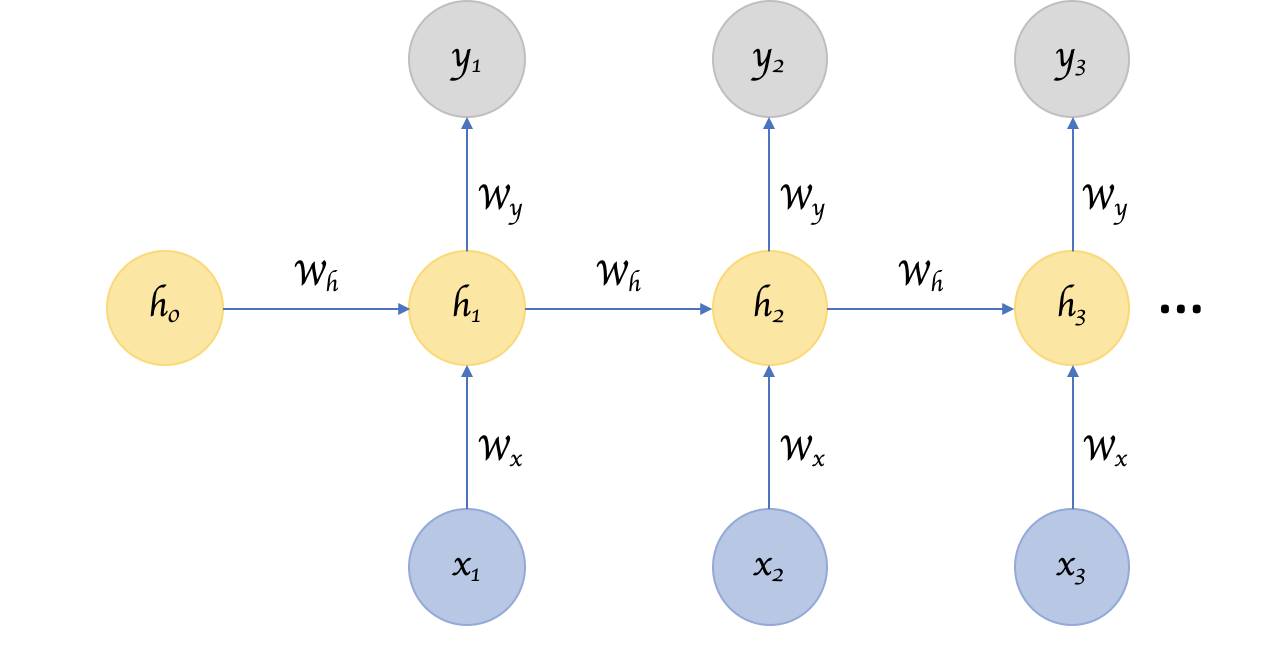
\includegraphics[width=0.75\textwidth]{recurrent-nn.png}
    \caption{Ілюстрація структури рекурентної нейронної мережі}
    \label{fig:rnn}
\end{figure}

Рішення рекурентної мережі, досягнуте на етапі часу $t-1$, впливає
на рішення, яке вона прийме через один шаг на етапі часу $t$.
Отже, рекурентні мережі мають два джерела вхідних даних -- поточні
та недавнє минуле, які разом визначають, як мережа
реагує на нові дані.

Можна сказати, що рекурентні зв'язки в нейронній мережі
дають можливість пам'ятати попередні рішення.
Додавання пам’яті до нейронних мереж має ціль: у самій послідовності
є інформація, і рекуррентні мережі використовують її для виконання
завдань, які мережі прямого зв'язку не можуть.
А саме, прихований стан дозволяє шукати
кореляційні залежності між подіями, розділеними багатьма моментами,
і ці кореляції називаються ``довгостроковими залежностями'',
оскільки подія за течією часу залежить і є функцією однієї
або кількох подій, що відбулися раніше.

Звичайна рекурентна одиниця описується формулами:

\vspace{0.5em}
\begin{gather}
\begin{aligned}
    h_t &= \phi(W_h h_{t-1}+W_x x_t+b)\\
    y_t &= h_t
\end{aligned}
\end{gather}
\vspace{\baselineskip}

Тут $x_t$ це вхід, $h_t$ -- рекурентна інформація, а $y_t$ -- 
результат на кроці $t$.

Однак рекурентні мережі, що складаються зі стандартних рекурентних
одиниць, не здатні обробляти довгострокові залежності: у міру
зростання розриву між відповідними входами важко
вивчити з'єднану інформацію. Основними причинами проблеми
довгострокових залежностей є те, що сигнали про помилки,
що надходять назад у часі, мають тенденцію або підірватися,
або зникнути \cite{nn:recurrent-hard}.

Для вирішення цієї проблеми було розроблено багато
методів, таких як LSTM \cite{nn:lstm}, GRU \cite{nn:gru}. Вони
гарно себе показали у задачах, які потребують захоплення
довгострокових залежностей. Такі задачі включають, але не обмежуються,
розпізнавання мови, машинний переклад.

Задачі, де завдання полягає у відображенні однієї послідовності в
іншу (машинний переклад, розпізнавання мови) становлять
виклик для рекурентних
нейронних мереж, оскільки вони вимагають, щоб розмірність
входів і виходів була відомою та фіксованою.
Для вирішення цієї проблеми була запропонована
модель ``seq2seq'' \cite{nn:seq2seq}. Загалом, вона спрямована
на перетворення вхідної послідовності (джерела) на нову (цільову),
і обидві послідовності можуть мати довільну довжину.
Приклади завдань трансформації включають машинний переклад
між кількома мовами як у тексті, так і в аудіо,
генерацію діалогу запитання-відповідь або навіть синтаксичний
розбір речень на дерева граматики.

Модель seq2seq зазвичай має архітектуру енкодер-декодер, що складається з:

\begin{enumerate}[label=--]
    \item Енкодер обробляє вхідну послідовність і стискає інформацію
    у контекстний вектор (також відомий як ембедінг речення
    або вектор ``думки'') фіксованої довжини. Очікується,
    що це відображення буде гарним підсумком значення
    цілої послідовності.
    \item Декодер ініціалізується контекстним вектором для
    виводу перетвореної послідовності. Ранні роботи
    використовували лише останній стан мережі
    енкодера як початковий стан декодера.
\end{enumerate}

І енкодер, і декодер є рекурентними нейронними мережами.

Критичним і очевидним недоліком цього дизайну контексту з
фіксованою довжиною є нездатність запам'ятовувати довгі речення.
Часто він забуває першу частину, як тільки завершує обробку всього
вводу. Для вирішення цієї проблеми народився
механізм уваги \cite{nn:attention}.

\section{Механізм уваги}
Увага до певної міри мотивована тим, як ми приділяємо зорову увагу
різним регіонам зображення або співвідносимо слова в одному реченні.

Зорова увага людини дозволяє зосередитись на певному регіоні з
``високою роздільною здатністю'', одночасно сприймаючи навколишнє
зображення в ``низькій роздільній здатності'', а потім відрегувати
фокусну точку або зробити відповідний висновок.
Враховуючи невеликий фрагмент зображення, пікселі в решті надають підказки, що
там відображається. Ми очікуємо побачити загострене вухо в жовтій коробці,
тому що ми бачили ніс собаки, ще одне загострене вухо праворуч і очі
Шіби (речі в червоних квадратах) (Рис. \ref{fig:shiba}). Однак
светр та ковдра внизу були
б не такими корисними, як ті собачі риси.

\begin{figure}[H]
    \centering
    
\includegraphics[width=0.75\textwidth]{shiba-example-attention.png}
    \caption{Шіба-іну в одязі}
    \label{fig:shiba}
\end{figure}

Подібним чином ми можемо пояснити зв'язок між словами в одному реченні
або близькому контексті. Коли ми бачимо ``їсти'', ми сподіваємось дуже
скоро зустріти слово, що означає вид їжи.

\begin{figure}[H]
    \centering
    
\includegraphics[width=0.75\textwidth]{sentence-example-attention.png}
    \caption{Одне слово ``поділяє увагу'' іншим словам по-різному}
    \label{fig:attend-example}
\end{figure}

Увагу при глибокому навчанні можна широко трактувати як вектор вагових
коефіцієнтів: для того, щоб передбачити або зробити висновок про один елемент,
наприклад, піксель на зображенні або слово в реченні, ми оцінюємо,
використовуючи вектор уваги, наскільки сильно він співвідноситься з іншими
елементами,
і приймає суму їх значень, зважену вектором уваги, як наближення
цілі \cite{attention}.

Механізм уваги народився, щоб допомогти запам’ятати довгі початкові
речення в машинному нейронному перекладі (МНП). Замість того,
щоб будувати єдиний вектор контексту із останнього прихованого стану
енкодера, підхід, винайдений увагою, полягає у створенні
скорочених шляхів між контекстним вектором та
всією вихідною послідовністю. Ваги цих з'єднань скорочення
можна підправити для кожного вихідного елемента.

Хоча вектор контексту має доступ до всієї початкової послідовності,
нам не потрібно турбуватися про забування.
Відповідність між джерелом та ціллю вивчається та контролюється
за допомогою контекстного вектора. По суті, вектор контексту
споживає три частини інформації:

\begin{enumerate}[label=--]
    \item прихований стан енкодеру;
    \item прихований стан декодеру;
    \item відповідність між входом та ціллю.
\end{enumerate}

\begin{figure}[H]
    \centering
    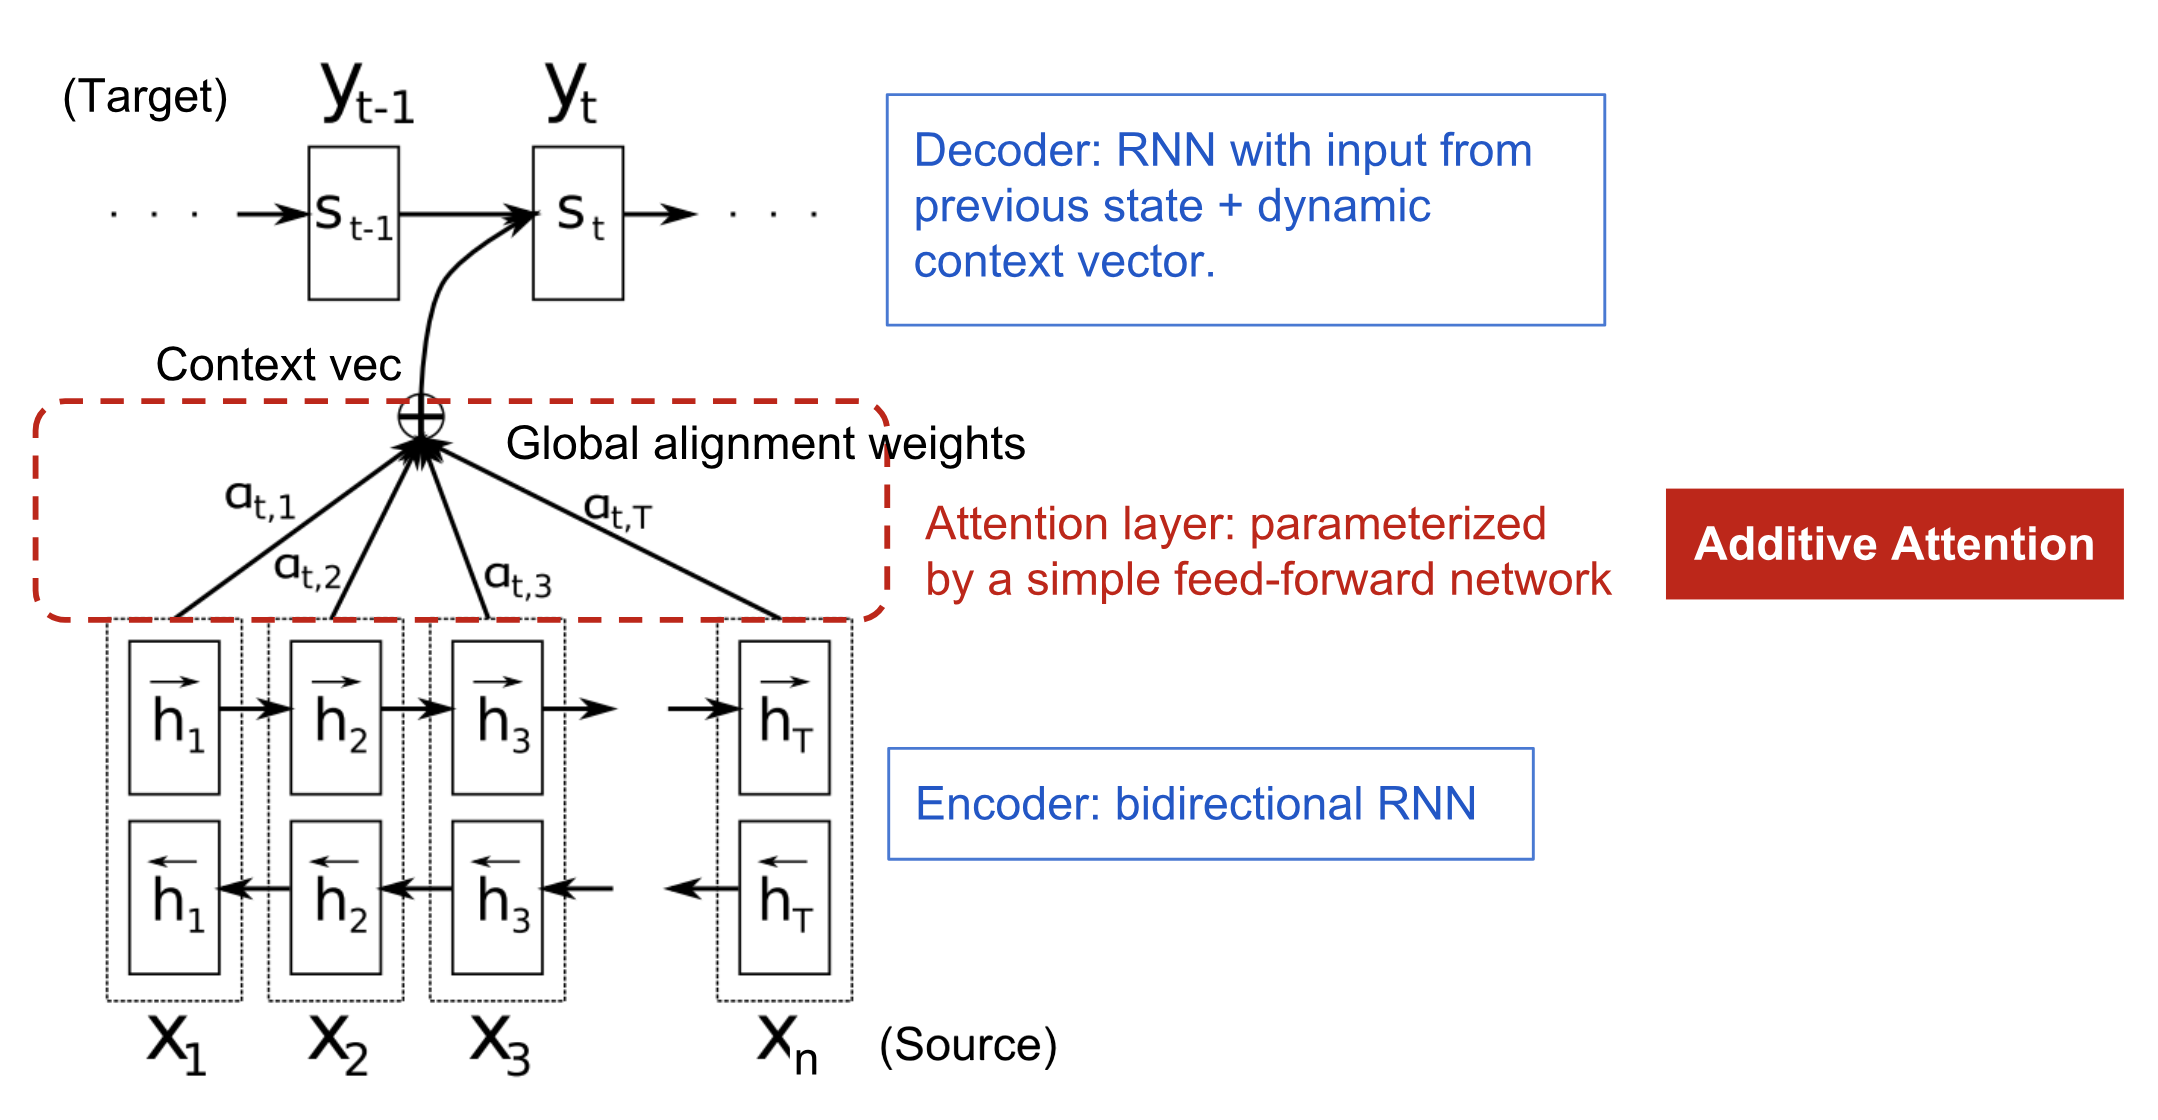
\includegraphics[width=1\textwidth]{encoder-decoder-attention.png}
    \caption{Архітектура рекурентної моделі з адитивною увагою}
    \label{fig:plot3}
\end{figure}

Механізм можна формально визначити так. Нехай є початкова послідовність
$x$ довжини $n$, і треба вивести цільову послідовність $y$
довжини $m$:

\vspace{0.5em}
\begin{gather}
\begin{aligned}
    x &= [x_1,x_2, ..., x_n] \\
    y &= [y_1,y_2, ..., y_n]
\end{aligned}
\end{gather}
\vspace{\baselineskip}

Тут енкодер -- це двонаправлена РНМ (або будь-яка інша РНМ) із прямим
прихованим станом $\overrightarrow{h_i}$ та зворотнім
$\overleftarrow{h_i}$. Звичайна конкатенація двох представляє стан
енкодера. Мотивація цієї операції
полягає в тому, щоб включити як попередні, так і наступні
слова до анотації одного слова.

\begin{equation}
    h_i = [\overrightarrow{h_i}^T;\overleftarrow{h_i}^T], i=1, ..., n
\end{equation}

Мережа декодера має прихований стан $s_t = f(s_{t-1},t_{t-1},c_t)$
для слова, що виводиться, на позиції $t$, $t = 1, ..., m$,
де контекстний вектор $c_t$ є сумою зважених прихованих станів
вхідної послідовності:

\vspace{0.5em}
\begin{gather}
\begin{aligned}
    c_t          &= \sum^n_{i=1}\alpha_{t,i} h_i \\
    \alpha_{t,i} &= \text{align}(y_t,x_t) \\
    &= \frac{\exp(\text{score}(s_{t-1}, h_i))}{\sum^n_{i'=1}\exp(\text{score}(s_{t-1},h_{i'}))}
\end{aligned}
\end{gather}
\vspace{\baselineskip}

Модель відповідності призначає оцінку $\alpha_{t,i}$
парі вхідних даних у позиції $i$ та виході у позиції $t$, ($y_t$, $x_i$),
залежно від того, наскільки вони співвідносяться. Множина
${α_{t,i}}$ -- це ваги, що визначають, наскільки кожен прихований стан
входу слід враховувати для кожного виводу.
У статті Багданау \cite{nn:attention} оцінка відповідності
$α$ параметризується мережею прямого пересилання
з єдиним прихованим шаром, і ця мережа навчається спільно з
іншими частинами моделі. Таким чином, функція оцінки
має такий вигляд, враховуючи, що $\tanh$ використовується як
нелінійна функція активації:

\begin{equation}
    \text{score}(s_t, h_i) = v^T_a \tanh(W_a [s_t;h_i])
\end{equation}
Де обидва $v_a$ та $W_a$ є матрицями вагів, які вивчаються
моделлю відповідності.

Існує декілька варіацій механізму
уваги \cite{attention:1} \cite{attention:2}, які змінюють
функцію вираховування відповідності. Вище
була використана аддитивна \cite{nn:attention} увага.

\section{Трансформери}
Робота ``Attention Is All You Need'' \cite{attention-all-need}
ввела архітектуру
``Трансформера'', яка була використана для задачі машинного
перекладу. Модель уникає необхідності використовувати
рекурентні з'єднання, та цілком полагається на
механізм уваги.

Основним компонентом трансформера є блок
багатоголовочної уваги. Трансформер розглядає закодоване
представлення входу як набір пар ключ-значення $(K, V)$,
обидва розмірності $n$ (довжина вхідної послідовності).
У декодері попередній вивід стискається у запит 
($Q$ розмірності $m$), а наступний вивід створюється
шляхом відображення цього запиту та набору ключів і значень.

Трансформер використовує масштабовану увагу
скалярного добутку: вихід є зваженою сумою значень,
де вага, що присвоєна кожному значенню, визначається
скалярним добутком запиту з усіма ключами:

\begin{equation}
    \text{Attention(Q,K,V)} = \text{softmax}(\frac{QK^T}{\sqrt{n}})V
\end{equation}

Де
\begin{equation}
    Q=XW_Q, K=XW_K, V=XW_V
\end{equation}

Тут $XW_Q, XW_K, XW_V$ це матриці ваг, які вивчаються
моделлю. $n$ це розмір матриці, який потрібен
для зменшення проблени зникаючих градієнтів \cite{attention-all-need}.

Важлимим компонентом трансформера є те, що
механізм самоуваги використовується декілька разів.
Замість того, щоб обчислити увагу лише один раз,
багатоголочна увага проходить через масштабовану увагу
скалярного добутку кілька разів паралельно. Виходи головок
уваги просто конкатенуються та лінійно перетворюються
до очікуваних розмірів. Це дозволяє різним голівкам
навчатися приділяти увагу різним речам.

\vspace{0.5em}
\begin{gather}
\begin{aligned}
    \text{MultiHead}(Q,K,V)= [\text{head}_1; ...; \text{head}_h]W^O \\
    \text{head}_i = \text{Attention}(QW^Q_i, KW^K_i, VW^V_i)
\end{aligned}
\end{gather}
\vspace{\baselineskip}

Де $QW^Q_i$, $KW^K_i$, $VW^V_i$ та $W^O$ -- матриці вагів,
які модель вивчає під час тренування.
Множення конкатенованого вектору на матрицю $W^O$
дозволяє накладати шари багатоголовочної уваги друг на друга,
тим самим збільшуючи силу представлення моделі, та дозволяючи
їй вивчати більш складні асоціації між словами.
Ілюстрацію багатоголовочного механізму уваги можна
побачити на рисунку \ref{fig:trans-multihead}.

\begin{figure}[H]
    \centering
    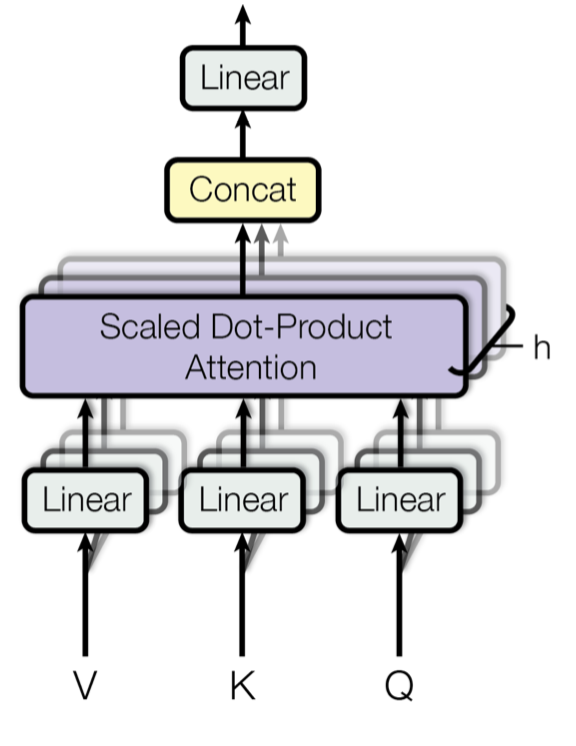
\includegraphics[width=0.35\textwidth]{multi-head-attention.png}
    \caption{Ілюстрація багатоголовочного механізму уваги}
    \label{fig:trans-multihead}
\end{figure}

Архітектура трансформера зі статті ``Attention Is All You Need''
використовувалась для задачі машинного перекладу, де
стандартна архітектура складається з енкодера, та декодера.
Енкодер створює представлення вхідного
потенційно-безкінечного контексту
на основі механізму уваги, а декодер витягує закодовану інформацію,
та виконує поточне завдання. Повна архітектура трансформера
є на рисунку \ref{fig:trans-arch}.

\begin{figure}[H]
    \centering
    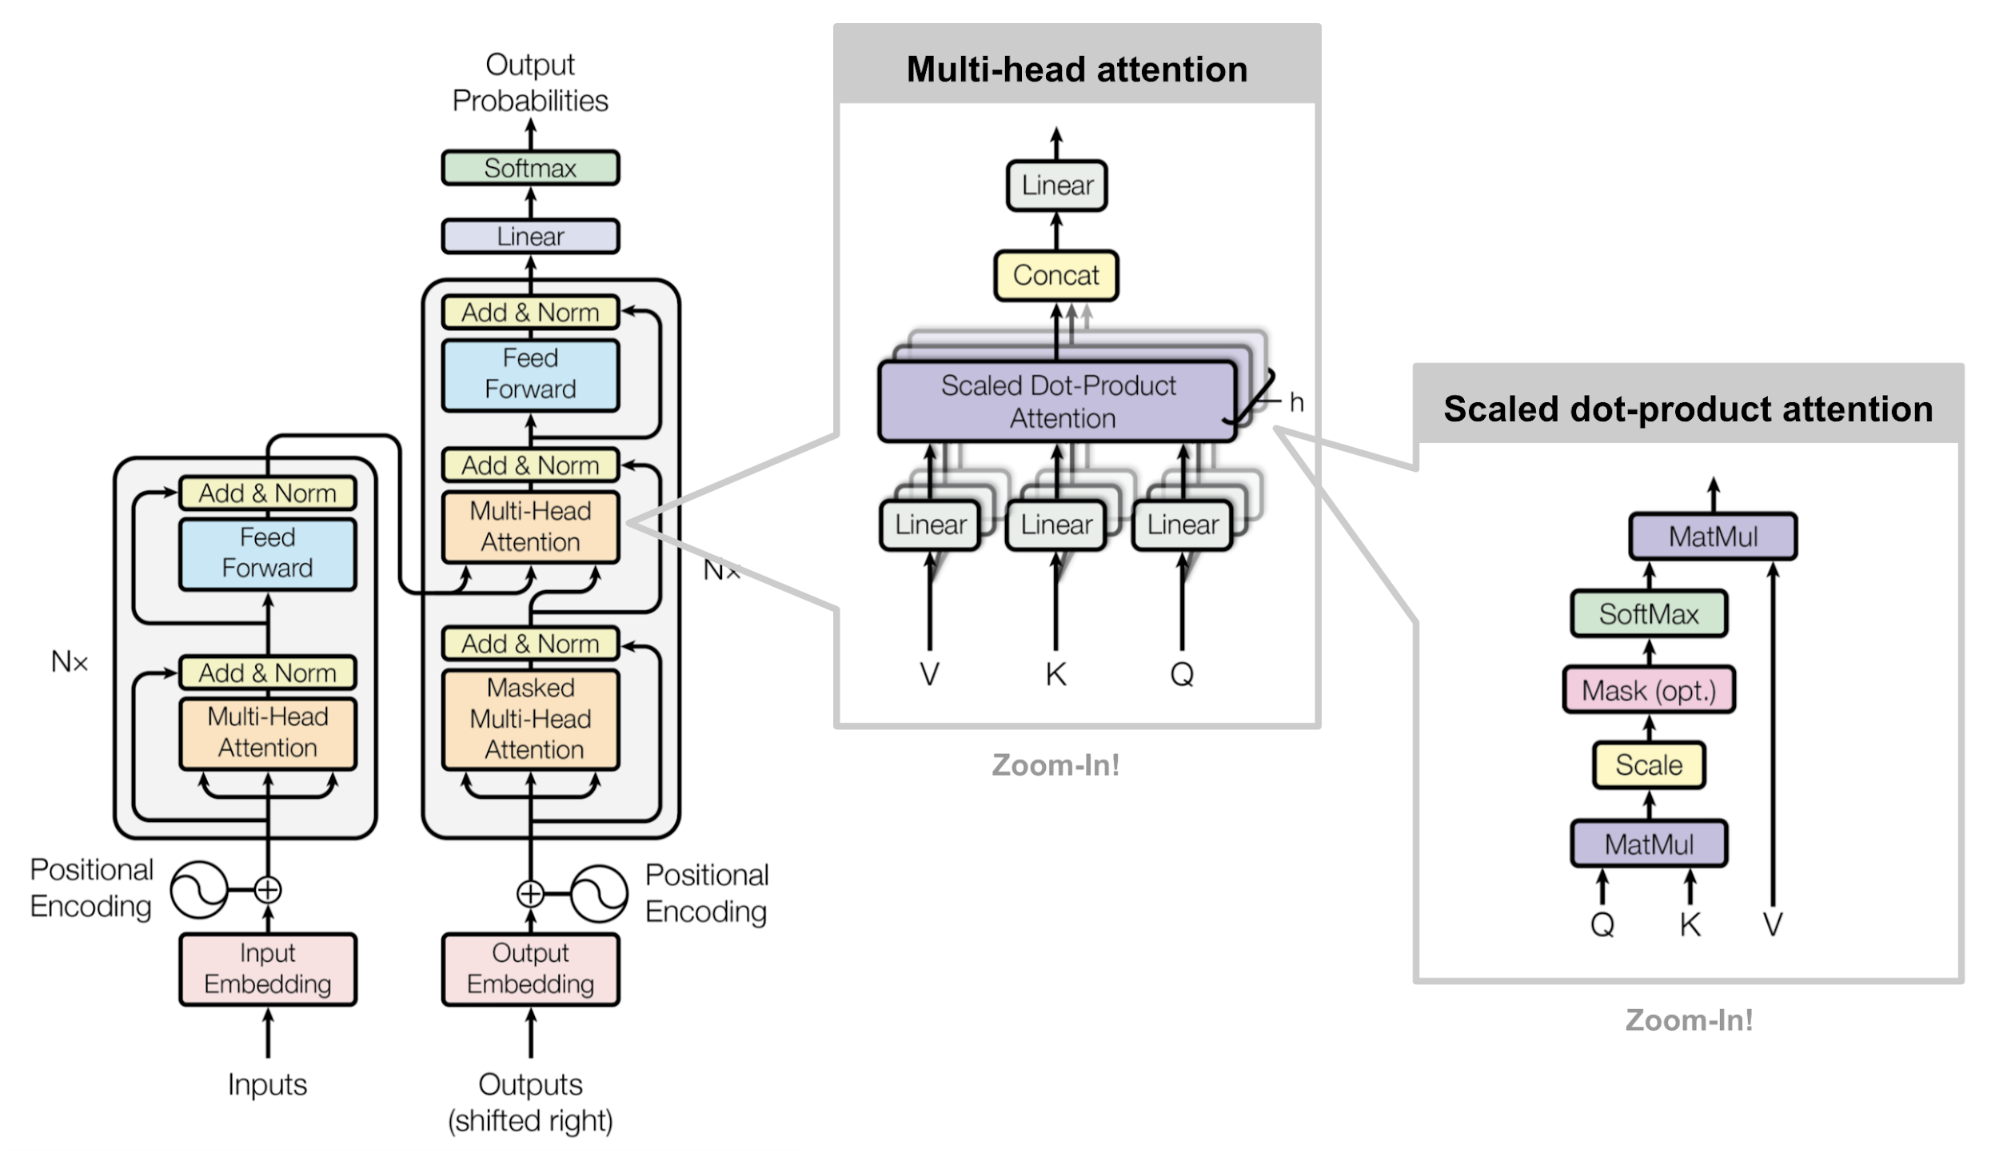
\includegraphics[width=1\textwidth]{transformer.png}
    \caption{Повна архітектура моделі трансформера}
    \label{fig:trans-arch}
\end{figure}

Таким чином, архітектури, засновані на трансформерах
уникають використання рекурентності у нейронних мережах і замість
цього цілком довіряють механізмам самоуваги для
вирішення задач, які традиційно найкраще вирішували
різні варіації рекурентних мереж.

\section{Постановка задачі}
Архітектура трансформер стала фактичним стандартом
для завдань з обробки природної мови, проте її застосування
до комп'ютерного зору залишається обмеженим. У комп'ютерному
зорі увага або застосовується разом із згортковими мережами (ЗНМ),
або використовується для заміни певних компонентів
згорткових мереж, зберігаючи загальну їх структуру на місці.

Задача цієї роботи полягає у застосуванні архітектури
трансформеру до задачі класифікації зображень. Ми хочемо показати,
що залежність від згорткових мереж не є необхідною, і чистий
трансформер, що застосовується безпосередньо до послідовностей
клаптиків зображень, може дуже добре виконувати
завдання класифікації зображень.

\newpage
\chapter{Теоретичні дослідження}
\section{Попередня робота}
Трансформери були запропоновані \cite{attention-all-need}
для машинного перекладу, і з тих пір стали
найсучаснішим методом у багатьох задачах обробки природної
мови. Великі моделі на основі трансформерів
часто попередньо навчаються на великих корпусах, а потім
доопрацьовуються для виконання поставленого завдання:
BERT \cite{bert}, GPT \cite{gpt}.

У попередніх роботах були запропоновані методи, які об'єднують
рекурентні і згорткові шари в одній моделі, для виконання задач
багатоміткової класифікації \cite{nn:cnn-rnn}, опису зображень.
Трансформери завдяки механізму уваги можуть
замінити рекурентні та згорткові шари. Наївне застосування
уваги до зображень вимагало б, щоб кожен піксель приділяв
увагу кожному іншому пікселю. При квадратичній вартості відносно кількості
пікселів, це не практично щодо реальних розмірів
вхідних зображень. Таким чином, щоб застосувати
трансформери в контексті обробки зображень,
раніше було спробувано кілька наближень. Одним з них
було застосовування самоуваги лише в локальних
регіонах для кожного пікселя запиту, а не глобально \cite{image-trans}.
Такі локальні багатоголовкові блоки із самоувагою
можуть повністю замінити згортання \cite{local-regions-attention}.

Найбільш пов’язаною з нашою є модель \cite{cordonnier},
яка розділяє вхідне зображення на регіони розміром
$2 \times 2$ і зверху застосовує повну увагу. Ця робота
дуже схоже на нашу, проте наша робота йде далі,
демонструючи, що масштабна попереднє тренування
робить звичайні трансформери
конкурентоспроможними (або навіть кращими) із найсучаснішими ЗНМ.
Також, \cite{cordonnier} використовує маленький розмір
регіону $2 \times 2$, що не дозволяє використовувати модель
на занадто великих зображеннях, коли наша модель успішно обробляє
зображення середнього розміру.

\section{Метод}

При розробці моделі ми максимально точно дотримуємося
оригінального трансформера \cite{attention-all-need}.
Перевагою цього навмисно простого підходу
є те, що масштабовані архітектури трансформерів
для задач обробки природної мови (та їх ефективні реалізації)
можуть бути використані майже без модифікацій.

\begin{figure}[H]
    \centering
    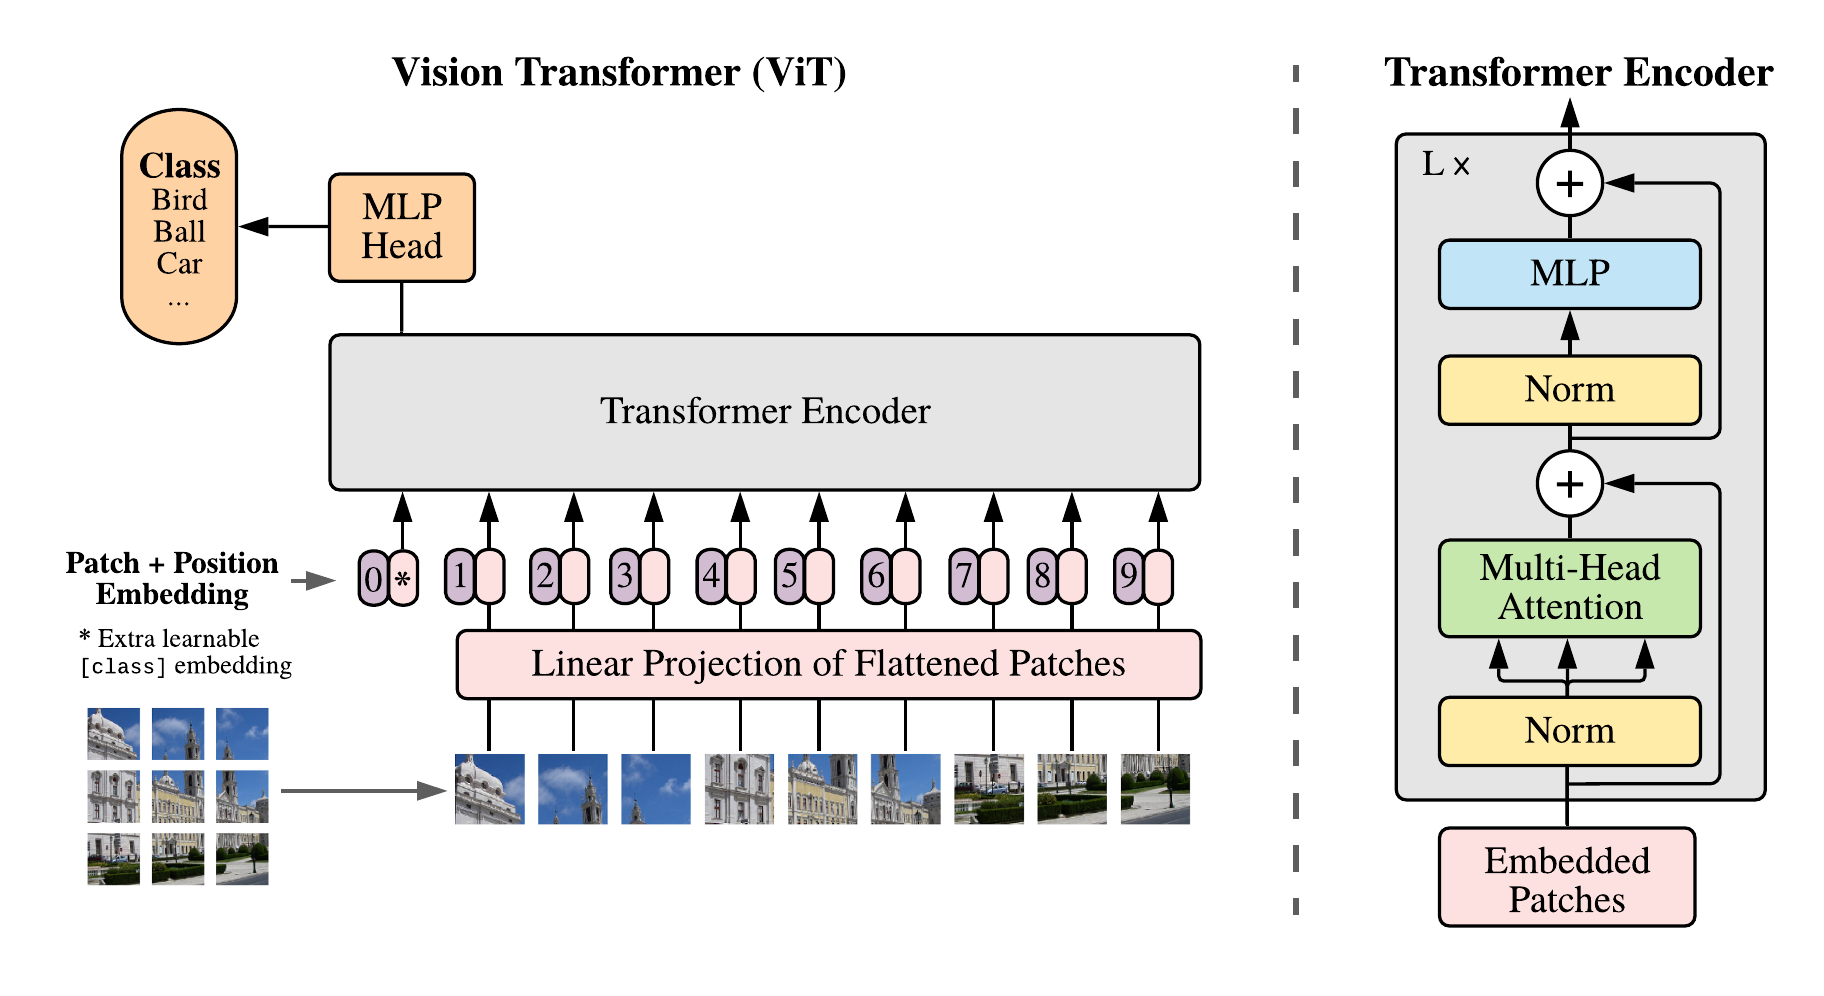
\includegraphics[width=1\textwidth]{vision-transformer-arch.png}
    \caption{Архітектура моделі}
    \label{fig:model-arch}
\end{figure}

\subsection{Vision Transformer}
Огляд моделі наведено на рисунку \ref{fig:model-arch}.
Стандартний трансформатор отримує на вхід 1D
послідовність ембедингів токенів.
Для обробки 2D-зображень ми змінюємо розмірність зображення
$x \in \mathbb{R}^{H\times W \times C}$ у послідовність
зплющених 2D регіонів $x_p \in \mathbb{R}^{N\times (P^2\cdot C)}$,
де $(H, W)$ -- роздільна здатність початкового
зображення, $C$ -- кількість каналів, $(P, P)$ -- роздільна
здатність кожного регіону зображення,
а $N = HW / P^2$ -- результуюча кількість регіонів,
яка також служить ефективною довжиною вхідної послідовності для
трансформера. Трансформер використовує
латентний векторний постійного розміру $D$ у всіх своїх шарах,
тому ми випрямляємо регіони та відображаємо у розмір $D$
за допомогою тренованої лінійної проекції (рівняння \ref{eq:1}).
Ми називаємо результат цієї проекції ембедінгами регіонів.

Так як ми працюємо не з послідовностями, ми додаємо
тренований ембедінг до послідовності ембедингів регіонів
$z_0^0 = x_{\text{class}}$. Його стан на виході енкодеру трансформера
($z_L^0$) служить як представлення зображення $y$ (рівняння \ref{eq:4}).
Як під час попереднього тренування, і під час точної настройки,
головка класифікації приєднана до  $z^0_L$.
Класифікаційна головка являє собою багатошаровий перцептрон
з одним прихованим
шаром під час попереднього тренування та одним лінійним шаром
під час точної настройки.

\begin{align}
    z_0 &= [x_{{class}};x_p^1 E;x_p^2 E; ...; x_p^N E] +E_{pos} \label{eq:1}\\
    E &\in \mathbb{R}^{(P^2 \cdot C)\times D},
    E_{pos} \in \mathbb{R}^{(N+1)\times D} \nonumber\\
    z'_l &= {MSA}({LN}(z_{l-1})) + z_{l-1}, &l=1...L \label{eq:2}\\
    z_l &= {MLP}({LN(z'_l)})+z'_l, &l=1...L \label{eq:3}\\
    y &= {LN}(z_L^0) \label{eq:4}
\end{align}

\section{Модель}
% In order to perform classification, we use the standard approach of adding an extra learnable “classification token” to the sequence.
% https://stackoverflow.com/questions/58123393/how-to-use-transformers-for-text-classification

\newpage
\chapter{ЕКСПЕРИМЕНТАЛЬНІ ДОСЛІДЖЕННЯ}
Ми оцінюємо можливості репрезентативного навчання
ResNet, Vision Transformer (ViT) та гібриду.
Щоб зрозуміти вимоги до даних кожної моделі, ми попередньо
тренуємось на наборах даних різного розміру та оцінюємо багато
контрольних завдань. Розглядаючи обчислювальні витрати на
попереднє тренування моделі, ViT працює дуже вигідно,
досягаючи кращих методів за більшістю тестів розпізнавання
за нижчої вартості попереднього тренування. Нарешті, ми проводимо
невеликий експеримент, використовуючи самоконтроль,
і показуємо, що самоувага ViT є перспективною.

\section{Налаштування}
\subsection{Датасети}
Для дослідження масштабованості моделі ми використовуємо
набір даних ILSVRC-2012 ImageNet з 1 тис. класами та 1,3 млн. зображеннями
(далі ми називаємо його ImageNet), його надмножину ImageNet-21k
з 21 тис. класами та 14 млн. зображеннями та JFT з 18 тис. 
класів та 303 млн. зображень із високою роздільною здатністю.
Ми видаляємо дублікати даних попередньої підготовки
відносно тестових наборів даних поточних завдань.
Ми переносимо моделі, навчені цим набором даних, на кілька базових завдань:
ImageNet на оригінальних мітках перевірки та очищених мітках ReaL,
CIFAR-10/100, Oxford-IIIT Pets та Oxford Flowers-102.

\subsection{Варіанти моделі}
Ми базуємо конфігурації ViT на тих, що використовуються для
BERT \cite{bert}, як описано в таблиці \ref{tab:t1}.
Моделі ``Base'' та ``Large'' безпосередньо беруться від BERT,
і ми додаємо більшу модель ``Huge''. Далі ми використовуємо
короткі позначення для позначення розміру моделі
та розміру вхідного регіону: наприклад, ViT-L/16 означає ``Large''
варіант із розміром вхідного патча $16 \times 16$.
Зауважте, що довжина послідовності трансформера
обернено пропорційна квадрату розміру регіона,
тому моделі з меншим розміром патча обчислювально дорожчі.

Для базових CNN ми використовуємо ResNet,
але замінюємо шари пакетної нормалізації
на групову нормалізацію і використовуємо стандартизовані згортки.
Для гібридів ми подаємо проміжні репрезентації у ViT з
розміром регіона один ``піксель''.

\begin{table}[H]
    \caption{Деталі варіантів моделі}
    \begin{tabular}{ c c c c c c }
        \hline
        Модель & Шари & Прихов. розмір $D$ & Розм. щільн. шару & Голов. & Парам.  \\ \hline
        ViT-Base & 12 & 768 & 3072 & 12 & 86M  \\ 
        ViT-Large & 24 & 1024 & 4096 & 16 & 307M  \\ 
        ViT-Huge & 32 & 1280 & 5120 & 16 & 632M  \\ \hline
    \end{tabular}
    \label{tab:t1}
\end{table}

\subsection{Навчання та точне налагодження}
Ми тренуємо всі моделі, включаючи ResNet, за допомогою Adam
з $\beta_1 = 0.9$, $\beta_2 = 0.999$, пеакетний розмір 4096 та вагою розпаду
$0.1$. Для точкого налагодженн ми використовуємо SGD з імпульсом,
розмір пакету 512, для всіх моделей.

\section{Порівняння з кращими сучасними методами}
Спочатку ми порівнюємо наші найбільші моделі 
-- ViT-H/14 та ViT-L/16 --
із найсучаснішими CNN з літератури. Першим пунктом порівняння є
Big Transfer (BiT) \cite{big-transfer}, який виконує навчання
з вчителем для переходу з великими ResNets.
Другий - Noisy Student, який є великим EfficientNet, який навчається
за допомогою напівконтрольного навчання на ImageNet та JFT-300M зі
знятими мітками. В даний час Noisy Student є найсучаснішим на
ImageNet та BiT-L для інших наборів даних, про які повідомляється тут.
Усі моделі пройшли навчання на апаратному забезпеченні TPUv3,
і ми повідомляємо про кількість днів, ядер TPUv3, необхідних
для попереднього тренування кожного з них, тобто про
кількість ядер TPU v3 (2 на чіп), помножених на час навчання в днях.

У таблиці \ref{tab:t2} наведені результати.
Менша модель ViT-L/16, попередньо навчена на JFT-300M,
перевершує BiT-L (яка попередньо навчена на тому самому наборі даних)
у всіх завданнях, вимагаючи при цьому значно менших обчислювальних
ресурсів для навчання. Більша модель, ViT-H/14, додатково покращує
продуктивність, особливо на більш складних наборах даних
-- ImageNet, CIFAR-100 та наборі VTAB. Цікаво, що модель все ще
вимагала значно менших обчислень для попереднього тренування,
ніж попередні сучасні моделі. Нарешті, модель ViT-L/16, попередньо
навчена на загальнодоступному наборі даних ImageNet-21k, також
добре працює на більшості наборів даних, при цьому вимагає 
менше ресурсів для попередньго тренування.

\begin{table}[H]
    \caption{Порівняння з кращими сучасними методами (1)}
    \begin{tabular}{ c c c }
        \hline
         & Ours-JFT (ViT-H/14) & Ours-JFT (ViT-L/16)  \\ \hline
        ImageNet           & 88.55 & 87.76  \\ 
        ImageNet ReaL      & 90.72 & 90.54   \\ 
        CIFAR-10           & 99.50 & 99.42  \\ 
        Oxford-IIIT Pets   & 94.55 & 93.90  \\ 
        Oxford Flowers-102 & 97.56 & 97.32  \\ 
        VTAB (19 задач)    & 99.68 & 99.74  \\ \hline
        TPUv3-core-days    & 77.63 & 76.28  \\ \hline
    \end{tabular}
    \label{tab:t2}
\end{table}

\begin{table}[H]
    \caption{Порівняння з кращими сучасними методами (2)}
    \begin{tabular}{ c c }
        \hline
         & Ours-121k (ViT-L/16)  \\ \hline
        ImageNet           & 85.30   \\ 
        ImageNet ReaL      & 88.62   \\ 
        CIFAR-10           & 99.15   \\ 
        Oxford-IIIT Pets   & 93.25   \\ 
        Oxford Flowers-102 & 94.67   \\ 
        VTAB (19 задач)    & 99.61   \\ \hline
        TPUv3-core-days    & 72.72   \\ \hline
    \end{tabular}
    \label{tab:t3}
\end{table}

\begin{table}[H]
    \caption{Порівняння з кращими сучасними методами (3)}
    \begin{tabular}{ c c c }
        \hline
         & BiT-L (ResNet152x4) & Noisy Student (EfficientNet-L2)  \\ \hline
        ImageNet           & 87.54 & 88.4  \\ 
        ImageNet ReaL      & 90.54 & 90.55  \\ 
        CIFAR-10           & 99.37 & --  \\ 
        Oxford-IIIT Pets   & 93.51 & --  \\ 
        Oxford Flowers-102 & 96.62 & --  \\ 
        VTAB (19 задач)    & 99.63 & --  \\ \hline
        TPUv3-core-days    & 78.29 & --  \\ \hline
    \end{tabular}
    \label{tab:t4}
\end{table}

\section{Огляд Vision Transformer}
Щоб почати розуміти, як Vision Transformer обробляє дані
зображення, ми аналізуємо його внутрішні уявлення. Перший шар
Vision Transformer лінійно проектує розгорнуті плями в простір
нижчих розмірів (рівняння \ref{eq:1}).
На рисунку \ref{fig:filters} (зліва) показано основні
компоненти вивчених фільтрів ембедингу.
Компоненти нагадують правдоподібні базові функції
для низьковимірного представлення тонкої структури в кожному
регіоні.

\begin{figure}[H]
    \centering
    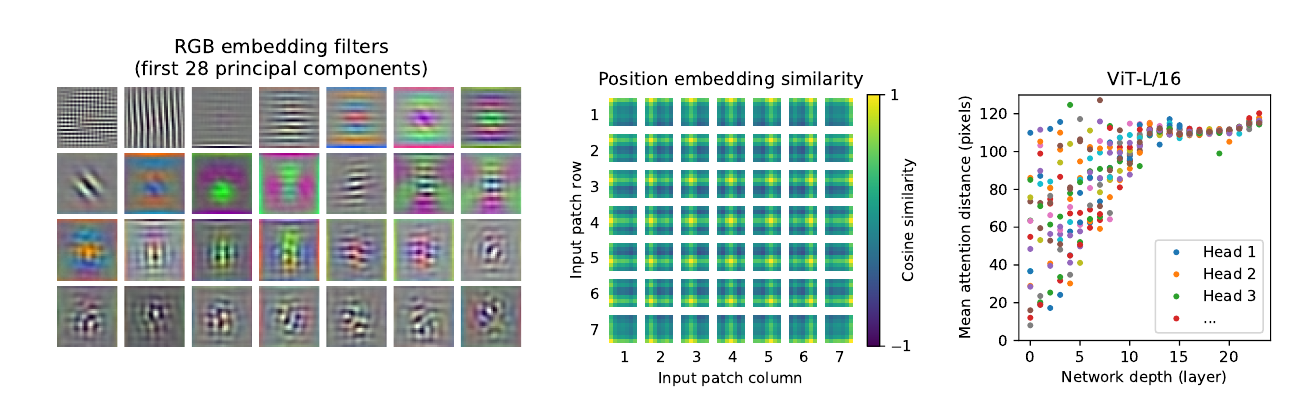
\includegraphics[width=1\textwidth]{filters.png}
    \caption{Фільтри початкового лінійного ембедингу, схожість позиційних ембедингів, розмір площі, якій головка приділяє увагу}
    \label{fig:filters}
\end{figure}

Після проекції до представлення регіонів зображення додається
позиціонний ембедінг. Рисунок \ref{fig:filters} (в центрі) показує,
що модель вчиться кодувати відстань всередині зображення за схожістю
позиційних ембедингів, тобто ближчі регіони, як правило, мають більше
подібних позиційних ембедингів. Далі з'являється структура рядка-стовпця;
регіони в одному рядку/стовпці мають подібні ембедінги.
Нарешті, синусоїдальна структура іноді виявляється для більших сіток.
Те, що позиційні ембедінги вчаться представляти
топологію 2D-зображень, пояснює, чому власноруч
створені 2D варіанти ембедингів не дають
вдосконалення.

Самоувага дозволяє ViT інтегрувати інформацію по всьому
зображенню навіть у найнижчих шарах. Ми досліджуємо, наскільки мережа
використовує цю можливість. Зокрема, ми обчислюємо середню
відстань у просторі зображення, через яку інтегрується інформація,
на основі ваг уваги (рисунок \ref{fig:filters}, праворуч).
Ця ``відстань уваги'' є аналогом розміру сприйнятливого поля в ЗНМ.
Ми виявили, що деякі головки придають увагу більшій частині зображення
вже на найнижчих шарах, показуючи, що модель справді
використовує здатність інтегрувати інформацію глобально.
Інші головки уваги мають постійно малі відстані уваги в низьких шарах.
Ця сильно локалізована увага менш виражена у гібридних моделях,
які застосовують ResNet перед трансформером
(Рисунок \ref{fig:filters}, праворуч), що припускає, що він може
виконувати подібну функцію, як ранні згорткові шари в ЗНМ.
Далі, відстань уваги зростає із збільшенням глибини мережі.
Глобально ми виявили, що модель враховує області зображень,
які є семантично важливими для класифікації
(рисунок \ref{fig:attention-repr}).

\begin{figure}[H]
    \centering
    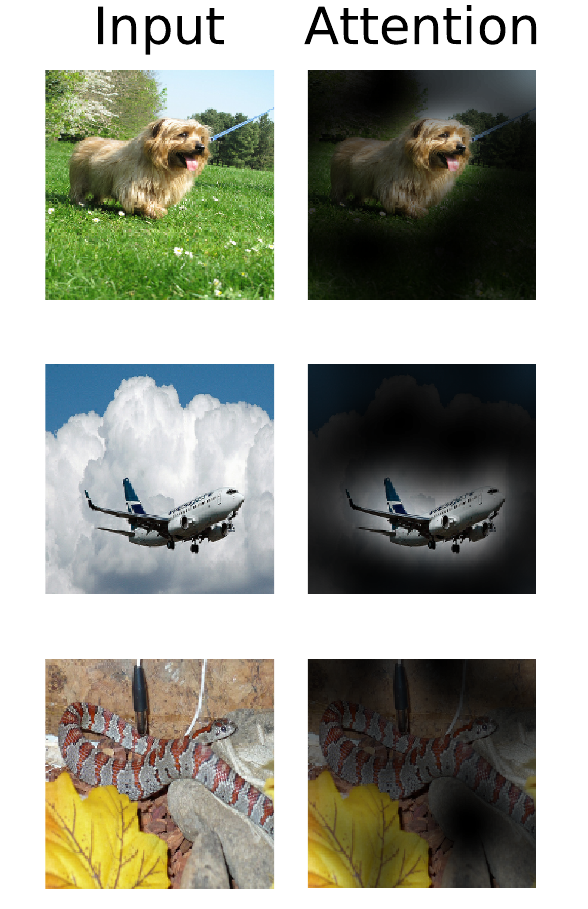
\includegraphics[width=0.3\textwidth]{attention-repr.png}
    \caption{Приклади уваги з вихідного токену то вхідного простору}
    \label{fig:attention-repr}
\end{figure}


\uchapter{ВИСНОВКИ}
Ми дослідили безпосереднє застосування трансформерів для розпізнавання
зображень. На відміну від попередніх робіт з використанням
самоуваги в комп'ютерному зорі, ми не вводимо специфічні для
зображень індуктивні зміщення до
архітектури, крім початкового етапу вилучення регіонів.
Натомість ми інтерпретуємо зображення як послідовність регіонів
і обробляємо його за допомогою стандартного енкодера трансформеру,
який використовується в задачах обробки природної мови.
Ця проста, але масштабована стратегія напрочуд добре працює у поєднанні
з попереднім тренуванням на великих наборах даних.
Таким чином, Vision Transformer відповідає чи перевищує сучасні найкращі
моделі на багатьох наборах даних класифікації зображень,
хоча є відносно дешевим для попереднього тренування.
\cite{image-worth-16-16-words}

Ми провели аналіз предметної галузі, теоретичні дослідження,
та експериментальні дослідження. Значна частина теоретичних
та практичних досліджень були взяті з чудової статті
``An Image is Worth 16x16 Words: Transformers for Image
Recognition at Scale''
В ній розглядається нова архітектура, яка може класифікувати
зображення без використання згорткових шарів, на основі трансформера.
Трансформери на поточний час є найкращими архітектурами для
задач обробки природної мови, та обїодяться без рекурентних
з'єднань. Так як трансформери не використовують ні рекурентність,
ні згортковість, а значним обмеженням цих підходів є
необхідність роводити обчислення послідовно, то трансформери
можуть оброблювати кожен вхід незалежно та паралельно,
що значно зменшує обчислювальні потреби. Таким чином,
у розглянутій статті трансформер застосовується до
нового домену (класифікація зображень), та, використовуючи
великі обчислювальні здатності багатьох TPUv3, веревершує
найкращі сучасні методи. Треба зазначити, що трансформер --
це більш загальна модель, ніж РНМ та ЗНМ, тобто
для того щоб досягти або перевершити методи
з сильним вбудованним в архітектуру індуктивним зміщенням,
треба набагато більше даних, щоб досягти того ж самого результату.
Перевагою трансформерів перед іншими методами полягає в тому,
що якщо даних дуже багато, то його можна тренувати
ефективніше, та він буде давати кращій результат, ніж інші методи.
Розглянута стаття доторкається до цієї проблеми, та розглядає
окремий етап ``попереднього тренування'', який полягає у
попередньому навчанні на великих датасетах, та точному налаштуванні
для вирішення поточної задачі.

Отже, більш загальні моделі -- трансформери -- можуть успішно
використовуватися для вирішення задач обробки зображень, якщо
є достатньо даних та обчислювальних ресурсів.

\newpage
\renewcommand\bibname{ПЕРЕЛІК ДЖЕРЕЛ ПОСИЛАННЯ}
\begin{thebibliography}{9}
    \bibitem{latex:friends}
    What are TeX and its friends? [Електронний ресурс] – Режим доступу до ресурсу: https://www.ctan.org/tex.

    \bibitem{latex:oss-devs-latex}
    Gaudeul A. Do Open Source Developers Respond to Competition? The LATEX Case Study / Alex Gaudeul. // Review of Network Economics. – 2007.

    \bibitem{webhooks:define}
    Webhooks [Електронний ресурс]. – 2019. – Режим доступу до ресурсу: https://developer.atlassian.com/server/jira/platform/webhooks/.

    \bibitem{webhooks:good}
    Lindsay J. Web hooks to revolutionize the web [Електронний ресурс] / Jeff Lindsay. – 2007. – Режим доступу до ресурсу: https://web.archive.org/web/20180630220036/http://progrium.com/blog/2007/05/03/web-hooks-to-revolutionize-the-web/.
    
    \bibitem{transformers:repo}
    State-of-the-art Natural Language Processing for Jax, PyTorch and TensorFlow [Електронний ресурс] – Режим доступу до ресурсу: https://github.com/huggingface/transformers.

    \bibitem{flashtext:arxiv}
    Replace or Retrieve Keywords In Documents at Scale [Електронний ресурс]. – 2017. – Режим доступу до ресурсу: https://arxiv.org/abs/1711.00046.

    \bibitem{flashtext:repo}
    FlashText module [Електронний ресурс] – Режим доступу до ресурсу: https://github.com/vi3k6i5/flashtext.

    \bibitem{ahocorasik:wiki}
    Aho–Corasick algorithm [Електронний ресурс] – Режим доступу до ресурсу: https://en.wikipedia.org/wiki/Aho%E2%80%93Corasick_algorithm.

    \bibitem{attention}
    Weng L. Attention? Attention! [Електронний ресурс] / Lilian Weng // lilianweng.github.io/lil-log. – 2018. – Режим доступу до ресурсу: http://lilianweng.github.io/lil-log/2018/06/24/attention-attention.html.

    \bibitem{cortex-stuff}
    Hubel D. Receptive fields, binocular interaction and functional architecture in the cat’s visual cortex / D. Hubel, T. Wiesel. // The Journal of physiology. – 1962. – С. 106–154.

    \bibitem{cortex-equations}
    Hodgkin A. quantitative description of membrane current and its application to conduction and excitation in nerve / A. Hodgkin, A. Huxley. // The Journal of physiology. – 1952. – С. 500–544.

    \bibitem{rozenblatt}
    Rosenblatt F. The perceptron, a perceiving and recognizing automaton Project Para / Frank Rosenblatt. // Cornell Aeronautical Laboratory. – 1957.

    \bibitem{nn:peyre}
    Peyré G. Mathematics of Neural Networks [Електронний ресурс] / Gabriel Peyré – Режим доступу до ресурсу: https://mathematical-tours.github.io/book-basics-sources/neural-networks-en/NeuralNetworksEN.pdf.

    \bibitem{nn:backpropagation}
    Rumelhart D. Learning representations by back-propagating errors / D. Rumelhart, G. Hinton, R. Williams. // nature. – 1986. – С. 533–536.

    \bibitem{gradient-descend}
    Ruder S. An overview of gradient descent optimization algorithms / Sebastian Ruder. // arXiv preprint arXiv:1609.04747. – 2016.

    \bibitem{nn:multilayer-perceptrons}
    Grosse R. Lecture 5: Multilayer Perceptrons [Електронний ресурс] / Roger Grosse – Режим доступу до ресурсу: https://www.cs.toronto.edu/~mren/teach/csc411\_19s/lec/lec10\_notes1.pdf.
\end{thebibliography}

\newpage
\chapter*{ДОДАТОК А}
\addcontentsline{toc}{chapter}{Додатки}
\centerline{Програмна реалізація}
\vspace{\baselineskip}
\inputminted[breaklines,linenos=true]{python}{untitled0.py}

% \newpage
% \section*{Додаток 1}
% \centerline{\uppercase{\bf{Програмна реалізація}}}
%     \inputminted[breaklines,linenos=true]{python}{../../src/app.py}

% \chap{Додаток 2}
% \centerline{\uppercase{\bf{Результати роботи}}}
%     \begin{figure}[H]
%         \centering
%         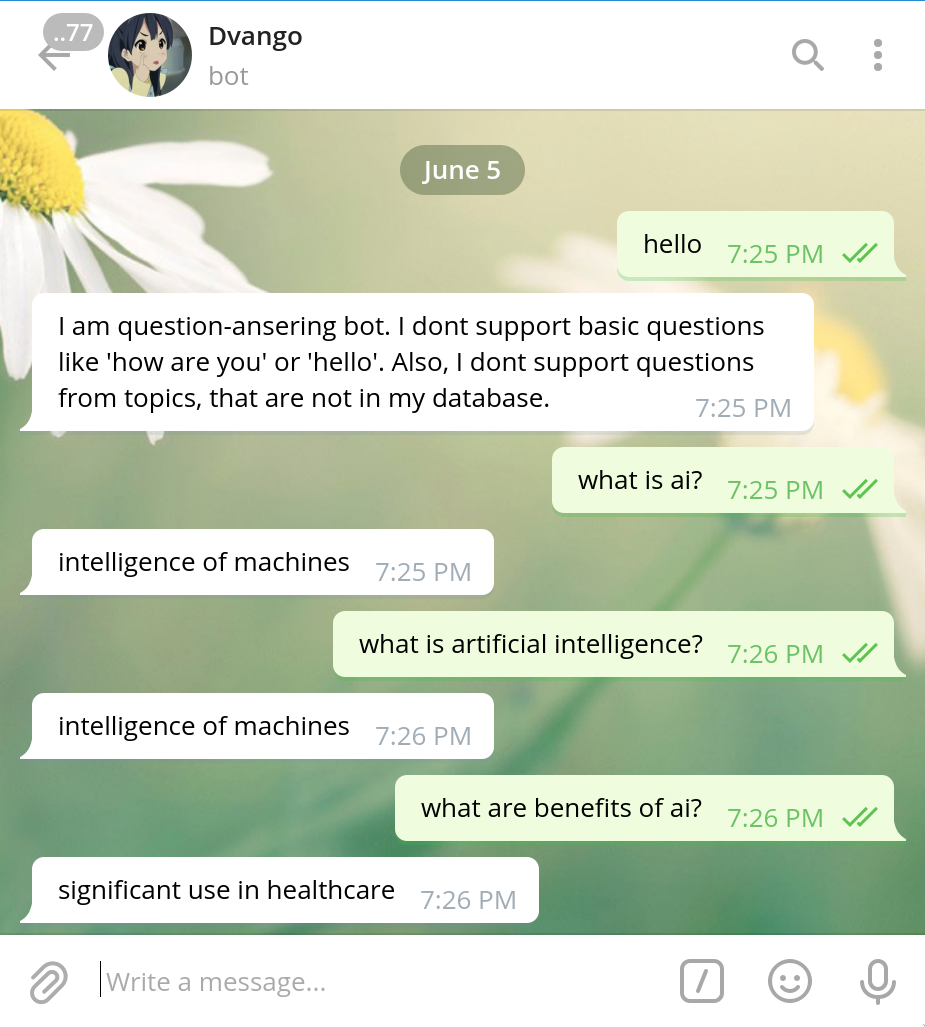
\includegraphics[width=0.75\textwidth]{f1.png}
%     \end{figure}
    
%     \begin{figure}[H]
%         \centering
%         
\includegraphics[width=0.75\textwidth]{f2.png}
%     \end{figure}

%     \begin{figure}[H]
%         \centering
%         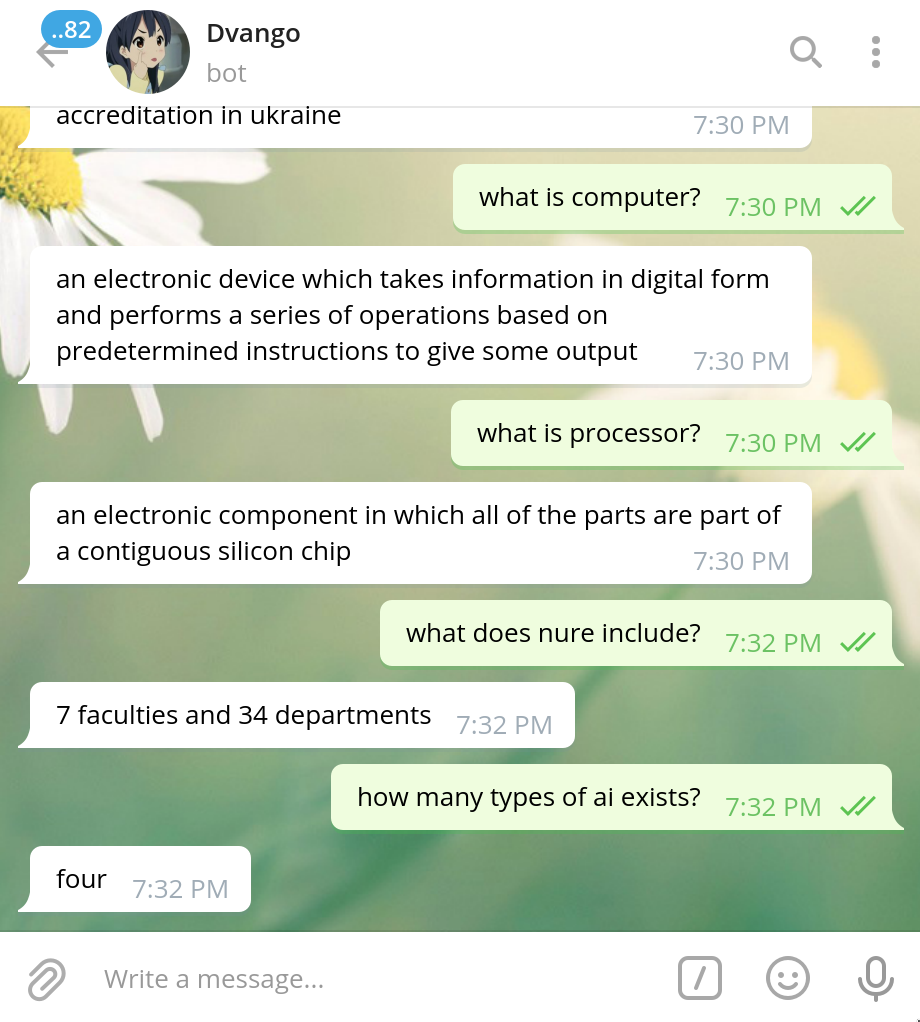
\includegraphics[width=0.75\textwidth]{f3.png}
%     \end{figure}
\end{document}


% \begin{figure}[H]
%     \centering
%     \includegraphics[width=0.75\textwidth]{rplot_iris.png}
%     \caption{Графік дерева вибірки Iris з дискретизацією через IG}
%     \label{fig:plot3}
% \end{figure}

% \begin{table}[H]
%     \centering
%     \begin{tabular}{ |c|c|c|c| } 
%      \hline
%      Мова   & \multicolumn{3}{c|}{Метод та датасет} \\ \hline
%             & Iris Thr. & Iris IG & SUSY \\ \hline
%      Python & 0.9333    & 0.9333  & 0.6799 \\ \hline
%      R      & 0.9333    & 0.9777  & 0.6594 \\ 
%      \hline
%     \end{tabular}
%     \caption{Порівняння точності класифікації}
%     \label{tab:t1}
% \end{table}
% \inputminted[breaklines,linenos=true]{scilab}{repl235.txt}
